%%%%                %%%%
%%%% IMPLEMENTACIÓN %%%%
%%%%                %%%%

\chapter{Diseño e Implementación}
\label{chap:implemetación}

\lettrine{E}{ste} capítulo describe el diseño y la implementación de la solución construida. El sistema implementa un flujo de datos que para el que se ha recurrido a tres lenguajes de programación, Python, C y Bash.

\section{Etapas del sistema}

Los datos son sometidos a un proceso por etapas tal como se ve en \ref{vision-general-del-sistema}. A continuación se detalla cada una de estas etapas.

\begin{figure}[hp!]
    \centering
    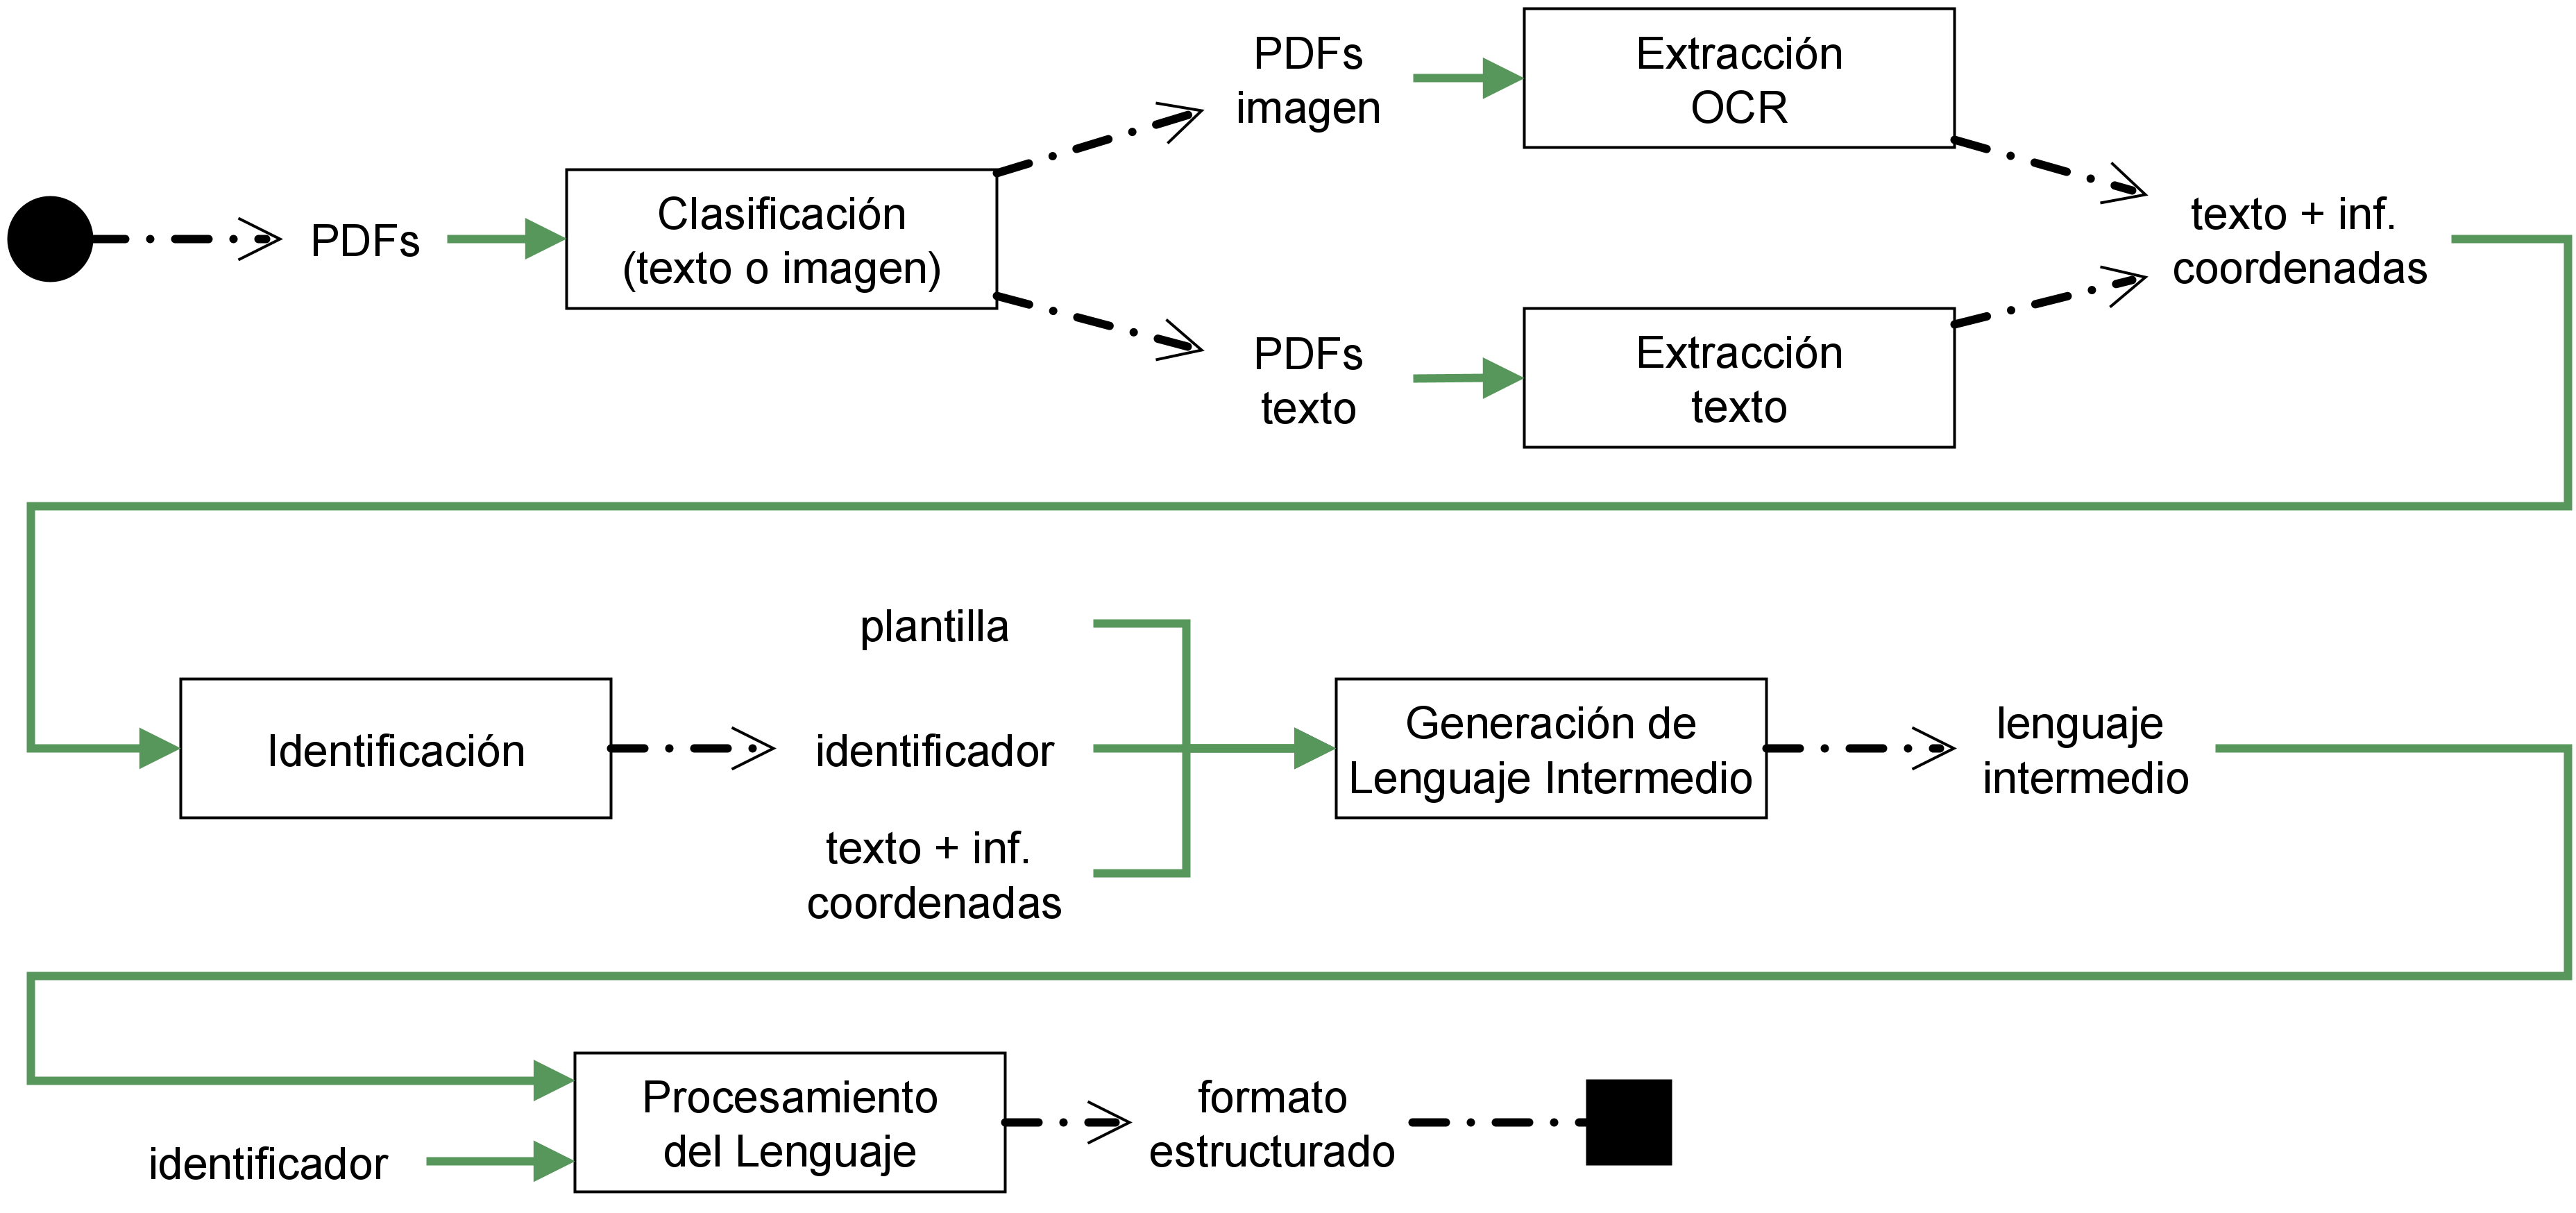
\includegraphics[width=1.0\textwidth]{imaxes/h-implementacion/vision-general-del-sistema-2}
    \caption{Visión general del sistema}
    \label{fig:vision-general-del-sistema}
\end{figure}

% TODO descripción del diagrama
% TODO en la aplicación se mantiene el estado interno por medio del sistema de ficheros

\subsection{Clasificación de los ficheros}

Los PDF recibidos deben ser clasificados dependiendo de su contenido. En unos casos es posible utilizar directamente el texto del documento para los restantes se procederá a utilizar el software OCR.

% TODO explicar en detalle como se hace la diferenciación


\subsection{Extracción de datos}

% TODO separación de las páginas individuales

% TODO comentar caso con pdftotext
% TODO incluir flags utilizados
% TODO ejemplo de salida de la información

% TODO comentar caso con OCR
% TODO parámetros de Tesseract
% TODO para cumplir con el requisito de tiempo reducido de ejecución se configuró Tesseract para emplear todos los cores disponibles en la máquina
% TODO ejemplo de salida de la información

\subsection{Identificación}

% TODO modelo de identificación. Explicar que está pensado para ser extensible a uso de BD u otras fuentes de información
% TODO explicar como se recorre el array en bash
% TODO mostrar la lista de identificadores
% TODO mostrar como se marca el directorio con el fichero .id

\subsection{Plantillas y regiones}
% TODO Tipos de regiones
% TODO información contenida en las plantillas (la que no se refiere a coordenadas)

\subsection{Generación del lenguaje intermedio}
% TODO describir la implementación en etapas, como el diagrama general
    % TODO Concepto de línea de identificación
    % TODO Asignación de palabras a regiones
    % TODO información de bounding box
% TODO mostrar el código intermedio
% TODO introducir el problema de indentificar las líneas
% TODO explicar se utiliza el algoritmo de Hough en los ejemplos donde es efectivo
% TODO explicar mejora en el algoritmo para asignación de palabras a regiones para cumplir con el requisito no funcionar de mantener los tiempos contenidos

\subsection{Procesamiento del lenguaje intermedio}
% TODO explicar como es la estructura general de Flex / Bison
% TODO mostrar las modificaciones introducidas
% TODO explicar la carga dinámica de librerías
% TODO Mencionar que el modelo de plugins permite entregar al cliente solo los modelos comprados
% TODO mostrar como es el formato de un fichero Flex y también Bison
% TODO Mostrar como se utiliza la librería para generación de ficheros JSON
% TODO Mencionar el pretty printing con jq

\section{Creación de un engine modular}
% TODO Se imita un modelo de procesamiento en batch
% TODO Se generan códigos de identificación de los jobs recibidos. También marca final.
% TODO Estructura de directorios considerada
% TODO Flujo de la información
% TODO explicar como es el flujo de información y por qué los terminales y no terminales llevan un tipo de dato en Bison

\section{Compilación y despliegue}

\subsection{Makefile}
% TODO mostrar el Makefile

\subsection{Ansible}
% TODO mostrar script Ansible

\subsection{Docker}
% TODO Mostrar fichero de configuración Docker y su uso

% TODO valorar si incluir capítulo o sección de pruebas. O, al menos, de pruebas realizadas.

\section{Editor de coordenadas}

